\documentclass{article}
\usepackage{import}
\subimport{../}{preamble}
\begin{document}

\section{Improved Field Enhancement of Spherical Au Nanoparticle Tips}

A result of spherical Au tips sustaining plasmon resonances which couple with the far-field is that their plasmonic contribution to the field enhancement can outperform the lightning rod contribution in sharp tips (assuming no near-field plasmonic excitation in sharp tips). The field enhancements for both sharp and spherical Au tips, more specifically the fabricated AuNP-on-Pt tips, are determined in a far-field side illumination configuration by using Raman scattering.

\begin{figure}[bt]
\centering
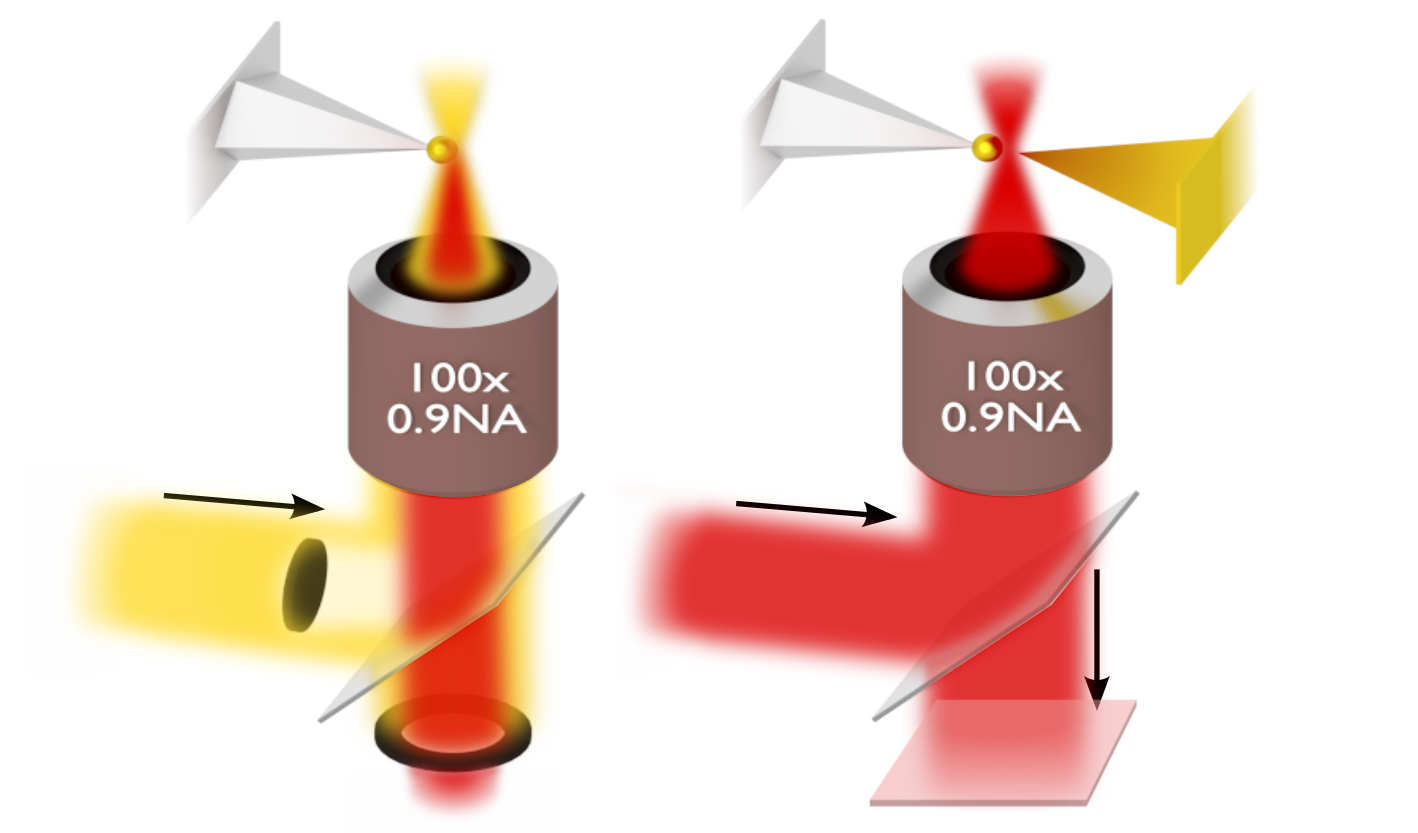
\includegraphics[width=0.55\textwidth]{figures/ters_setup}
\caption[Experimental geometry for dark-field spectroscopy and SERS measurements]{\textbf{Experimental geometry for dark-field spectroscopy and SERS measurements.} A \SI{125}{nm} radius spherical AuNP grown onto a Pt-coated AFM tip is spectroscopically studied using a supercontinuum laser in a dark-field configuration. The tip is then brought within \SI{1}{nm} of a benzenethiol-coated sharp Au tip under \SI{638}{nm} illumination to measure SERS spectra.}
\label{fig:ters_setup}
\end{figure}

% Introduction to the method and experiment configuration
Supercontinuum dark-field spectroscopy is used in conjunction with Raman spectroscopy in a modified version of the microscope platform, enabling both techniques. Fabricated AuNP AFM tips are mounted opposite a benzenethiol-coated sharp Au AFM tip in a tip-to-tip configuration, mimicking a plasmonic bow-tie antenna (\figurename~\ref{fig:ters_setup}). This configuration is used to obtain good optical access to the dimer gap for spectroscopically probing its plasmonic properties. Benzenethiol (BTh) is used as a Raman marker for measuring the relative field enhancement of AuNP tips due to its strong Raman response and well-known spectra \cite{mahajan2009, dudin2010}.
% BTh coating method
BTh (VWR International Thiophenol for synthesis) is diluted to \SI{5}{mM} solutions into ethanol (Sigma-Aldrich). Tips for use as SERS substrates are prepared by coating a monolayer of BTh onto the surface. This is achieved by submerging a standard Au-coated AFM tip in \SI{100}{mM} ethanolic BTh solution for \SI{1}{\minute} followed by rinsing with ethanol and drying in nitrogen. This is repeated 5 times to ensure complete monolayer coverage. Tips for use as plasmonic probes are not coated in BTh.

% Experimental TERS/characterisation procedure
With the BTh tip retracted, dark-field apex scattering spectra of tips is acquired using the supercontinuum laser source. After characterisation the microscope optics are modified into a TERS configuration and the plasmonic probe tip is aligned to the BTh tip using the capacitive tip alignment technique.%
\footnote{The optics are modified in the sense that the laser input is switched and the dark-field iris is opened.}
Once aligned, the gap size is reduced to  $\sim$\SI{1}{nm}, limited by the thickness of the assembled BTh molecular layer, and illuminated through a $100\times$ 0.9\,NA visible objective with \SI{3}{mW} (\SI{1.9}{\mega\watt\per\centi\metre\squared}) of \SI{638}{nm} laser light incident on the gap,  polarised along the tip axis. Scattered light is collected through the same objective and confocally localised. Raman spectra are filtered using a \SI{650}{nm} long-pass filter prior to dispersion in a spectrometer. Contact dynamics, confirming that tips come into physical contact, while separated by a BTh layer are measured using in-built AFM laser deflection from the cantilever of the approaching tip.

% Simulations
Near-field calculations for the spherical Au tip are computed for comparison with experimental results and to understand the enhancement mechanism. The near-field distribution at \SI{633}{nm} and the spectrum \SI{1}{nm} from the apex are calculated using the full electrodynamic boundary-element method \cite{deabajo1997, deabajo2002}.%
\footnote{Near-field calculations carried out by Lars O. Herrmann.}
The spherical tip is modelled as a Pt cone with half-angle \SI{20}{\degree} with a \SI{250}{nm} diameter AuNP attached to its end. The neck radius between sphere and tip is \SI{50}{nm}. The tip is illuminated with a plane wave polarised along the tip axis.

\begin{figure}[bt]
\centering
\begin{tikzpicture}
\node [below right] at (0,0) {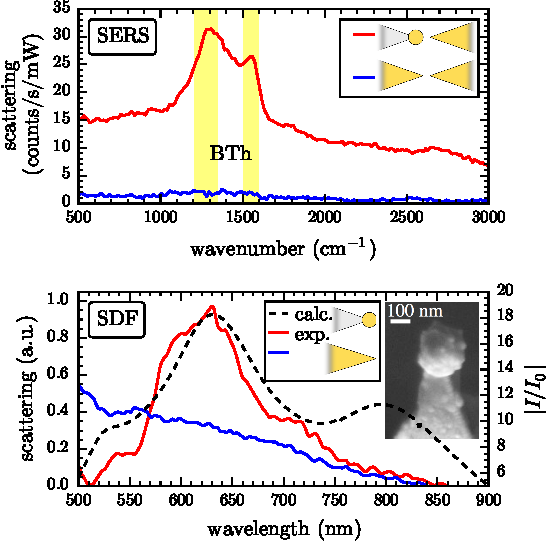
\includegraphics{figures/ters_comparison}};
\node [right] at (0,-0.2) {(a)};
\node [right] at (0,-5.0) {(b)};
\node [below right] at (9.5,-0.1) {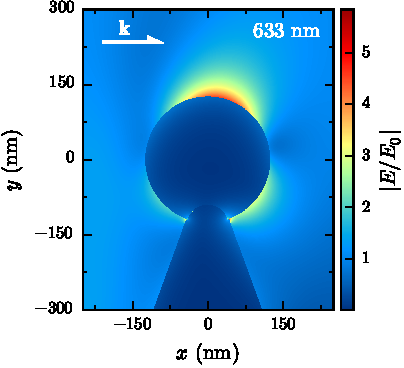
\includegraphics{figures/aunp_tip_nearfield}};
\node at (9.9,-0.2) {(c)};
\end{tikzpicture}
\caption[Application of sharp Au and AuNP-on-Pt tips to enhancing Raman scattering]{\textbf{Application of sharp Au and AuNP-on-Pt tips to enhancing Raman scattering.}
%\caption[Comparative TERS and dark-field spectroscopy of sharp Au and AuNP tips]{
(a,b) Comparative TERS and dark-field spectroscopy of sharp Au and AuNP tips. (a) Tip-enhanced Raman spectra of a benzenethiol-coated Au AFM probe brought close to the AuNP tip (red), compared to a sharp Au AFM tip (blue). (b) Dark-field optical scattering of AuNP (red) and sharp Au (blue) AFM tips, with calculated relative intensity enhancement \SI{0.5}{nm} from the AuNP tip apex (dashed). The inset shows an SEM image of the \SI{125}{nm} AuNP tip. %}
%\caption[Calculated field enhancement profile for a \SI{125}{nm} radius AuNP at the end of a \SI{1500}{nm} long Pt tip]{
(c) Calculated field enhancement profile for a \SI{125}{nm} radius AuNP at the end of a \SI{1500}{nm} long Pt tip. The neck join is \SI{50}{nm} wide and the tip is under longitudinally polarised plane wave illumination at \SI{633}{nm}.}
\label{fig:ters_comparison}
\end{figure}

%\begin{figure}[bt]
%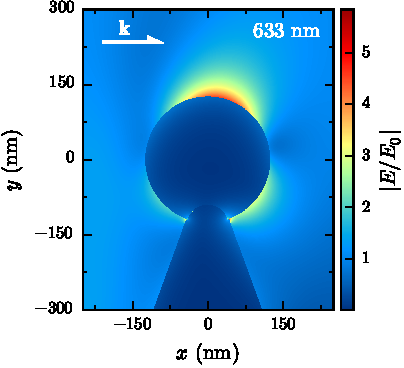
\includegraphics{figures/aunp_tip_nearfield}
%\caption[Calculated field enhancement profile for a \SI{125}{nm} radius AuNP at the end of a \SI{1500}{nm} long Pt tip]{\textbf{Calculated field enhancement profile for a \SI{125}{nm} radius AuNP at the end of a \SI{1500}{nm} long Pt tip.} The neck join is \SI{50}{nm} wide and the tip is under longitudinally polarised plane wave illumination at \SI{633}{nm}.}
%\label{fig:aunp_tip_nearfield}
%\caption[Application of sharp Au and AuNP-on-Pt tips to enhancing Raman scattering]{\textbf{Application of sharp Au and AuNP-on-Pt tips to enhancing Raman scattering.}}
%\end{figure}

A \SI{125}{nm} radius spherical AuNP-on-Pt tip, grown as described in section \ref{sec:initial_fabrication} (\SI{-8}{V}, \SI{150}{ms} exposure), is used to demonstrate the augmented plasmonic properties of spherically nanostructured tips. Raman spectra of BTh molecules in the tip dimer gap are greatly enhanced when using a AuNP tip in place of a sharp Au tip (\figurename~\ref{fig:ters_comparison}a). As the same spectrometer is used for both broadband scattering spectra and SERS spectra, its restricted spectral resolution (300--\SI{1100}{nm} bandwidth), combined with the broadness of the diode laser line illumination, blurs the characteristic multiple Raman peaks of BTh between 1000--\SI{1600}{\per\centi\metre}. However the resulting observation of two broad peaks in this region affirms the presence of BTh in the gap between tips. The background signal is also enhanced across a broad bandwidth, as is typical for SERS \cite{mahajan2009}.

Supercontinuum dark-field scattering spectra (\figurename~\ref{fig:ters_comparison}b), taken of individual tips prior to SERS measurements, show that the increased Raman enhancement when using a AuNP tip is due to excitation of a LSP around \SI{630}{nm}, not present in sharp Au tips. This is in good agreement with boundary element calculations of the near-field enhancement at the AuNP tip apex with a visible plasmon resonance observed across the AuNP (\figurename~\ref{fig:ters_comparison}b,c).
Coupling between this LSP in the AuNP tip with a BTh-coated sharp Au tip forms a confined gap plasmon mode. Since coupling is between higher order modes in the sharp Au tip, shifting of this resonance as a function of gap size is weak \cite{hugall2012}.%
\footnote{This needs checking}
Illuminating on resonance with the plasmon therefore greatly increases the Raman response by a factor of 30. This corresponds to a relative SERS enhancement of 12 when using a AuNP tip as opposed to a sharp Au tip after taking into account the confinement and mode volume of a LSP to the gap in each case \cite{romero2006}. Since the LSP is laterally confined to only \SI{7}{nm} within this gap the enhanced Raman signal is the result of scattering contributions from only a very small number of molecules. This leads to lower bound estimates for the absolute SERS enhancements of \num{1.9e5} for the AuNP tip and \num{1.6e4} for a sharp Au tip. Though absolute estimates are not as high as expected, the relative SERS enhancement observed with the AuNP tip is indeed comparable to previously reported results \cite{umakoshi2012}.

% Field enhancement calculations
Field enhancements are estimated by first calculating the mode volumes of plasmonic gap modes. The lateral width of a gap plasmon mode is given by $w=\sqrt{R_{\mathrm{eff}}d}$, where $R_{\mathrm{eff}}$ is the effective radius of the particles, $\sqrt{R_1R_2}$, comprising the plasmonic dimer and $d$ is the width of the gap separating particles \cite{romero2006}.%
\footnote{The use of $R_{\mathrm{eff}}=\sqrt{R_1 R_2}$ is justified by...}
This results in lateral mode widths of \SI{4.5}{nm} for the sharp Au tip of \SI{20}{nm} radius and \SI{7.1}{nm} for a \SI{125}{nm} AuNP tip.%
\footnote{Note that these widths are below the quantum limit for such large AuNPs only because the opposing tip has such a small radius to increase localisation.}
Assuming a cylindrical gap mode yields mode volumes of \SI{15.7}{nm\cubed} and \SI{39.3}{nm\cubed}, respectively. These define the near-field contribution to Raman scattering and a relative field enhancement is obtained using,
\begin{equation}
\mathit{FE}_{real} = \frac{N_{\mathit{AuNP}} / V_{\mathit{AuNP}}}{N_{\mathit{tip}} / V_{\mathit{tip}}}
\end{equation}
where $N$ is the Raman signal counts and $V$ is the mode volume. This evaluates to 12. Lower limit absolute field enhancements are estimated using,
\begin{equation}
\mathit{FE}_{abs} = \frac{N_{\mathit{near-field}} / V_{\mathit{near-field}}}{N_{\mathit{far-field}} / V_{\mathit{far-field}}}
\end{equation}
where $N_{\mathit{far-field}}$ is assumed to be \SI{0.1}{counts/s/mW} from the noise levels since signals are below the signal to noise level and $V_{\mathit{far-field}}$ is assumed to be \SI{25000}{nm\cubed} based upon the surface of a conical tip exposed to the focal volume of a diffraction limited spot ($d = \SI{412}{nm}$ at $\lambda = \SI{638}{nm}$). This expression yields absolute field enhancements of \num{1.9e5} for an \SI{80}{nm} AuNP tip and \num{1.6e4} for a sharp Au tip.

% Conclusions of plasmonic tips
These optical measurements confirm that AuNP tips provide increased field enhancement compared to sharp Au tips due to a strong LSP excitation. Lack of any strong peaks around \SI{600}{nm} in dark-field spectra of sharp Au tips suggest that any plasmons present are weakly coupled and do not scatter strongly in this illumination geometry. Such plasmons may still couple with the opposing tip to form a gap mode but reduced localisation results in a lower field enhancement. On the other hand, AuNP tips are well suited to high enhancements when illuminated at the appropriate plasmonic resonances.
Whilst a number of plasmonic probes have been developed recently, several useful features are obtained here. By using standard AFM probes as a basis, these AuNP tips maintain their functionality as AFM probes for force microscopy, as demonstrated by the alignment of tips using resonant capacitive driving. The metallic coating of these tips also allows for simultaneous electrical measurements whilst performing optical and AFM force measurements. These tips therefore function as standard electrical AFM probes with added plasmonic functionality.
Furthermore, such tips also show excellent resistance to damage at the tip apex after multiple surface contacts, though surfaces do become deformed after heavy use. Their robust nature is attributed to the direct growth of the AuNP root across the pyramidal tip end. This is a significant improvement over currently-available commercial spherical AFM tips, in which the spheres break from the tip and adhere to the contact surface after only one or a small number of contact cycles.

Several advantages emerge from apex-selective single nanoparticle electrochemical growth. Simultaneous nanoparticle growth on many tips ensures a high throughput process, while morphology and size is controlled by voltage and time. This provides a viable method for producing tips capable of expanding the user-base of plasmonics and furthering research into applications of TERS and SNOM. Further applications are envisaged, for instance in plasmonic optical trapping \cite{lindquist2013} because the tips in the present geometry can conveniently act as a heat sink reducing the problematic optical heating observed, and resulting thermal damage. Furthermore, the spherical nanoparticle growth method introduced here is not restricted to specific metals, and many different composite systems can be created with this apex-localised growth technique. For example silver nanoparticle tips give a larger optical response and field enhancement under visible illumination (although oxidation is sometimes an issue).

\end{document}